%
% char.tex -- graph of characteristics in problem 90000018
%
% (c) 2019 Prof Dr Andreas Müller, Hochschule Rapperswil
%
\documentclass[tikz,12pt]{standalone}
\usepackage{amsmath}
\usepackage{times}
\usepackage{txfonts}
\usepackage{pgfplots}
\usepackage{csvsimple}
\usetikzlibrary{arrows,intersections,math}
\begin{document}
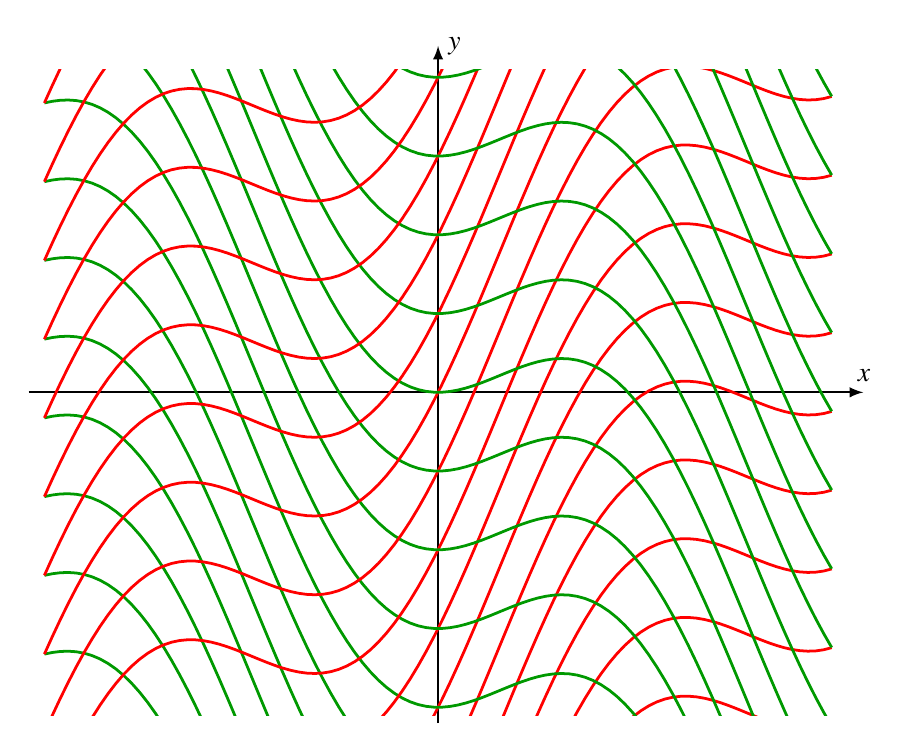
\begin{tikzpicture}[>=latex]

\definecolor{darkgreen}{rgb}{0,0.6,0}

\pgfmathparse{180/3.14159}
\xdef\s{\pgfmathresult}

\draw[->,line width=0.7pt] (-5.2,0)--(5.4,0) coordinate[label={$x$}];
\draw[->,line width=0.7pt] (0,-4.2)--(0,4.4) coordinate[label={right:$y$}];

\begin{scope}
\clip (-5.1,-4.1) rectangle (5.1,4.1);

\foreach \u in {-10,...,10}{

\draw[line width=1pt,color=red] plot[domain=-5:5,samples=100]
	({\x},{-cos(\s*\x)+sin(\s*\x)+\x+\u});
\draw[line width=1pt,color=darkgreen] plot[domain=-5:5,samples=100]
	({\x},{-cos(\s*\x)+sin(\s*\x)-\x+\u});

}

\end{scope}

\end{tikzpicture}
\end{document}

